\documentclass[a4paper]{article}

%% Language and font encodings
\usepackage[portuges]{babel}
\usepackage[utf8x]{inputenc}
\usepackage[T1]{fontenc}
\usepackage{eurosym}
\usepackage{tikz}
\usepackage{pdfcolparallel}
\usetikzlibrary{arrows,shapes,positioning,shadows,trees}

\tikzset{
every node/.style={draw,text width=2cm,drop shadow},
style1/.style= {rectangle, rounded corners=2pt, thin,align=center,fill=blue!30},
style2/.style= {rectangle, rounded corners=6pt, thin,align=center,fill=blue!60},
style3/.style= {rectangle,thin,align=left,fill=blue!60}
}

%% Sets page size and margins
\usepackage[a4paper,top=3cm,bottom=2cm,left=3cm,right=3cm,marginparwidth=1.75cm]{geometry}

%% Useful packages
\usepackage{amsmath}
\usepackage{graphicx}
\usepackage[colorinlistoftodos]{todonotes}
\usepackage[colorlinks=true, allcolors=blue]{hyperref}

\title{Gestão de Projetos}
\author{João Calhau, m36764}

\begin{document}
\maketitle

\vfill

\begin{figure}[!ht]
\centering

\includegraphics[width=120mm]{uni.png}
\end{figure}

\vfill

\newpage

\tableofcontents

\newpage

\section{Project Scope}
\paragraph{}

\noindent Este projeto tem como objetivo a criação de uma plataforma online de criação de web sites. Esta aplicação poderá ser acedida através de um dispositivo android. \\
A aplicação será composta por 2 partes, o frontend e o backend. O frontend será composto por uma interface, que será o que o utilizador vai ver quando abrir a aplicação e com o que poderá interagir com. O backend será composto por toda a lógica da aplicação, ou seja, será onde o hosting do servidor para os web sites será feito, onde os gestos do utilizador no ecrã serão traduzidos para código HTML5, linguagem a qual web sites usam hoje em dia e onde a gestão e utilização de uma simples base de dados será feita (caso o cliente queira guardar o seu trabalho para mais tarde). \\
Estima-se que serão precisos cerca de 7 meses para a conclusão deste projeto.\\

nota: Este projeto será maioritariamente desenvolvido na universidade de Évora (mas não está adicionada aos Stakeholders do projeto visto apenas se tratar do sitio onde a programação será feita) 

\section{Project Team}

A equipa de desenvolvimento será composta por 4 pessoas:
\begin{itemize}
\item João Calhau - Project Manager/Developer
\item José Maria - Main app developer
\item André Gouveia - Main app designer
\item Pedro Santos - Developer/Designer
\end{itemize}

\noindent As competências que se esperam do project manager são que consiga motivar o grupo a trabalhar melhor, resolver eventuais conflitos que haja entre os membros do grupo e tomar conta de todo o processo de gestão do projeto. Espera-se ainda que saiba mínimos de HTML5, SQL (ou qualquer outra linguagem de base de dados relacional) e Java (mais especificamente Android). \\
\noindent As competências que se esperam do José Maria são saber os mínimos necessários de HTML5, SQL (ou outra linguagem de base de dados relacional) e Java (mais especificamente, Android). \\
\noindent As competências que se esperam do André Gouveia são técnicas relativamente avançadas de design de interfaces e código HTML5, visto a interface vir a ser feita com base em código de web app. \\
\noindent As competencias que se esperam do Pedro Santos são, um bocado de tudo, visto este membro da equipa de desenvolvimento trabalhar em um pouco de tudo. \\

\noindent Cabe ao project manager planear as suas atividades, assim como as da sua equipa de desenvolvimento, delegar tarefas e responsabilidades, controlar as atividades dos membros da equipa e estabelecer metas e objectivos para si e para a equipa. O project manager pode ainda decidir, mais tarde, mudar a organização da equipa ou delegar funções extra a certos elementos do grupo, se achar necessário. \\
Cabe a um main app developer desenvolver o backend da aplicação, ou seja, cabe a estes individuos criar o tradutor para código HTML5, o server host e a base de dados. \\
Cabe a um main app designer, assim, desenvolver a frontend da aplicação, ou seja, a interface que permitirá o a criação do web site por parte do utilizador. \\
Um Developer/Designer tanto pode trabalhar no frontend como no backend, dependendo do que seja necessário. Por esta razão um Developer/Designer necessita de conhecimentos em ambos os pontos. \\
Durante o desenvolvimento desta aplicação espera-se também um desenvolvimento de cada membro da equipa, tanto a nível intelectual como a nível relacional, por isso na duração deste projeto o project manager tomará especial atenção a todos os membros do grupo de maneira a avaliar a sua evolução ao longo do projeto.\\

\noindent Nota: Cada elemento do grupo, trabalha apenas nos dias úteis de uma semana, ou seja, aos fins-de-semana estão por sua conta e podem fazer o que quiserem. Também não trabalham a feriados.

\newpage

\section{Stakeholders}

Os stakeholders deste projecto são:
\begin{itemize}
\item Todos os elementos da equipa de desenvolvimento, incluindo o project manager.
\item Todos os clientes que usarem Android e fizerem download desta aplicação da play store.
\item O sponsor do projeto, neste caso teria de ser um Business Angel que estivesse disposto a providenciar capital para dar um \textit{start-up} a este projeto.
\end{itemize}

\section{Information Systems}

Todas as semanas será organizada uma reunião com os membros da equipa de desenvolvimento para se falar do estado do projeto, se o desenvolvimento está a proceder sem problemas, caso contrario quais são esses problemas e de que maneira podem ser resolvidos. Para além das reuniões, o projeto será feito com ajuda do GitHub, plataforma esta que ajudará a distinguir o trabalho feito por cada membro da equipa e que permitirá a troca, fácil e rápida, de código entre os vários membros da equipa de desenvolvimento.

\section{Planning}
A única pessoa capaz de fazer alterações no projeto depois de ter começado é o project manager. O project manager, tem também, capacidade de alterar esta regra delegando alguém da equipa de desenvolvimento, se achar necessário. O tempo total do projecto é o mesmo do caminho critico, que podemos ver mais abaixo, e são 145 dias (Estes dias contam apenas os dias em que os elementos dos grupos trabalham, não conta com feriados e fins-de-semana).

\subsection{Work Breakdown Structure (WBS)}

\begin{tikzpicture}[remember picture, level 1/.style={sibling distance=40mm}, edge from parent/.style={->,draw}, >=latex]
\centering
\node[style1]{App for Android}
child {node[style2] (c1) {FrontEnd}}
child {node[style2] (c2) {BackEnd}}
child {node[style2] (c5) {App}}
child {node[style2] (c4) {Testes}};

\node [style3, below of = c1, xshift=15pt] (c11) {Recolher dados};
\node [style3, below of = c11] (c12) {Criar descrições};
\node [style3, below of = c12] (c13) {Criar Interface};

\node [style3, below of = c2, xshift=15pt] (c21) {Crirar BD};
\node [style3, below of = c21] (c22) {Criar tradutor};
\node [style3, below of = c22] (c23) {Criar server};

\node [style3, below of = c5, xshift=15pt] (c51) {Criar a app};
\node [style3, below of = c51] (c52) {Juntar BD};
\node [style3, below of = c52] (c53) {Juntar interface};

\foreach \value in {1,2,3}
  \draw[->] (c1.195) |- (c1\value.west);

\foreach \value in {1,2,3}
  \draw[->] (c2.195) |- (c2\value.west);
  
 \foreach \value in {1,2,3}
  \draw[->] (c5.195) |- (c5\value.west);
\end{tikzpicture}

\newpage

\subsection{PERT}

\begin{figure}[!ht]
\centering
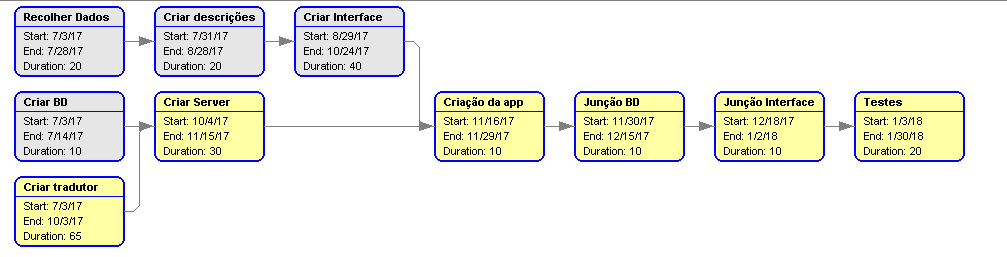
\includegraphics[width=120mm]{pert.png}
\caption{As atividades a amarelo são o caminho critico}
\end{figure}

\subsection{GANTT}

\begin{figure}[!ht]
\centering
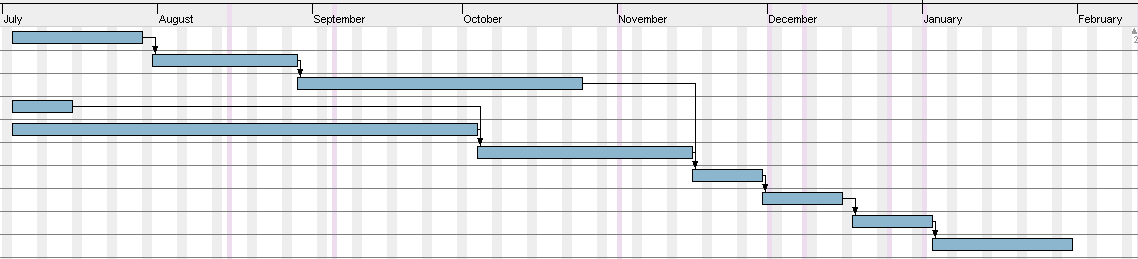
\includegraphics[width=120mm]{gantt.png}
\caption{Gráfico gantt do projeto}
\end{figure}

Lista de atividades do gráfico Gantt (por ordem):
\begin{itemize}
\item Recolher dados - 20 dias
\item Criar descrições - 20 dias
\item Criar interface - 40 dias
\item Criar BD - 10 dias
\item Criar tradutor - 65 dias
\item Criar server - 30 dias
\item criar app - 10 dias
\item Junção BD - 10 dias
\item Junção Interface - 10 dias
\item Testes - 20 dias
\end{itemize}

\newpage

\subsection{Resources}

\begin{figure}[!ht]
\centering
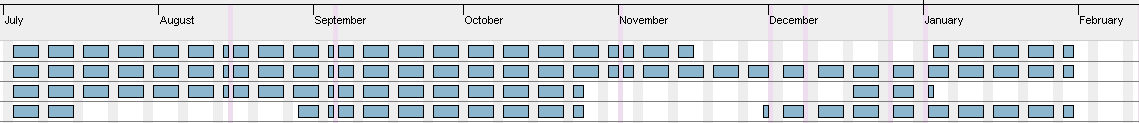
\includegraphics[width=120mm]{resurces.png}
\caption{Tabela de recursos}
\end{figure}

\section{Custos e Rentabilidade}

Os custos associados a este projeto serão o custo de registo como Developer na Google Play (25 euros), dois telefones Android OnePlus 3T, que têm um preço base de 439 euros, três computadores Asus ROG GL502VM, que tem um preço base de 1449 euros é ainda preciso um computador MSI WS63 7RK Workstation que tem um preço base de 2999 euros. Os Telefones servirão para fazer testes da aplicação à medida que esta vai sendo desenvolvida, os computadores serão usados para os 3 membros do grupo que irão fazer código e uma workstation para o André Gouveia que será quem se irá focar predominantemente em Design. Por isso no total serão precisos 7346 euros para começar o projeto, mais 878 euros quando se começarem a fazer os testes à aplicação e 25 euros para quando o trabalho estiver acabado e for para o meter na Google Play.

\begin{table}[!ht]
    \begin{tabular}{|c|c|c|c|c|}
    \hline
    ~                   & João Calhau & André Gouveia & José Maria & Pedro Santos \\ \hline
    Recolher Dados      & ~           & 100\%         & ~          & ~            \\ \hline
    Criar Descrições    & ~           & 100\%         & ~          & ~            \\ \hline
    Criar Interface     & ~           & 100\%         & ~          & 100\%        \\ \hline
    Criar BD            & ~           & ~             & ~          & 100\%        \\ \hline
    Criar Tradutor      & 100\%       & ~             & 100\%      & ~            \\ \hline
    Criar Server        & 100\%       & ~             & 100\%      & ~            \\ \hline
    Criar App           & ~           & ~             & 100\%      & ~            \\ \hline
    Juntar BD           & ~           & ~             & 100\%      & 100\%        \\ \hline
    Juntar Interface    & ~           & 100\%         & 100\%      & 100\%        \\ \hline
   	Testes              & 100\%       & ~             & 100\%      & 100\%        \\ \hline
    \hline
    \textbf{Material por pessoa}    & 1474\euro   & 2999\euro     & 1888\euro  & 1888\euro    \\ \hline
    \textbf{Custo por atividade} & 491.33\euro    & 749.75\euro   & 314.66\euro & 377.6\euro     \\ \hline
    \end{tabular}
\end{table}

Nota: Não há custos de mão de obra, visto que este projeto ser um projeto por conta própria. Assim como também não há pagamentos mensais ao grupo.\\

Para controlar este projeto, o project manager deve manter o projeto dentro dos objetivos programados durante o tempo da sua execução, estimular a pesquisa de soluções técnicas compatíveis com a qualidade adequada, detetar desvios entre o planeado e o real e ter conhecimento periódico do custo atual e custo final previsto do projeto durante o seu tempo de execução. 

\newpage

\subsection{Controlo de Custos}

Neste projeto o project manager vai ter de comparar custos de equipamentos reais, com os orçamentados (computadores e telefones), comparar a lista de materiais do orçamento com a lista final de materiais, adicionando a esta ultima os materiais que se irão introduzindo no projeto, caso sejam necessários, comparação dos custos de serviços (caso seja necessário dar host a um servidor permanentemente), estabelecer os custos de alteração durante o projeto. Será ainda necessária a escrita de um relatório com alterações do custo do projeto (este relatório só será feito quando estas alterações forem efetuadas).\\
Estas alterações, se necessárias, e a discussão sobre o estado financeiro do projeto será feita durante a reunião semanal falada mais cedo no projeto.

\section{Qualidade}

O objetivo principal da gestão da qualidade do projeto é assegurar que o projeto satisfaz as necessidades dos que lhe deram origem, portanto as dos Stakeholders, em especial as dos clientes. Se as especificações são atingidas e se o projeto estiver de acordo com as especificações técnicas e funcionais a qualidade do projeto dá-se assim como atingida. \\
De maneira a haver uma garantia da qualidade deste projeto, o project manager ter de avaliar periodicamente o desempenho do projeto. As pessoas encarreges de correr testes para ver se as atividades satisfazem os padrões de qualidade definidos, neste caso o project manager, o José Maria e o Pedro Santos, quando os estiverem a fazer têm de guardar os resultados dos testes de maneira a que na próxima reunião se possam discutir e, caso haja erros na aplicação, arranjar maneiras de os contrariar e fazer com que o programa fique com uma melhor qualidade no geral. Esta avaliação periódica, caso se desvie do planeado, será discutida nas reuniões semanais, mencionadas anteriormente.

\subsection{Especificações funcionais}
O intuito deste projeto é criar uma aplicação móvel que cria esqueletos de websites, o objetivo é criar esta aplicação em 125 dias com ajuda de mais três pessoas e depois pôr-la à venda por preço a discutir mais tarde, após trabalho estar feito, na Google Play Store. Como come esta aplicação o utilizador vai poder criar websites com um simples arrasto dos dedos esta aplicação vai ser útil a muitas pessoas que queiram criar um website, como por exemplo alguém que queira criar um website para vender produtos hortícolas mas não quer contratar alguém para fazer isso por ela, com esta aplicação basta fazer download e utilizar e temos um website em minutos.

\subsection{Especificações técnicas}
Os requisitos deste trabalho não são muitos, apenas se necessita de saber o mínimo de design (para a criação da interface), o mínimo de Android para a criação da aplicação Android e um pouco de HTML5, CSS e JavaScript para a tradução para os websites. É necessário ainda um pequeno conhecimento de Java, visto Android ser baseado em java.\\
Os materiais utilizados para a criação desta aplicação serão os computadores, que necessitarão de ter um disco minimamente bom e rápido para leitura e escrita de dados (SSD) e um disco para guardar uma grande quantidade de dados, não necessariamente rapidamente (HDD), precisariam ainda de um bom processador para processamento de dados, por isto os computadores escolhidos para este projeto foram os Asus ROG GL502VM. Para processamento de imagens e design em geral, o computador precisaria ainda de ter uma boa placa gráfica dedicada a processamento de imagem e por isso o escolhido foi a Workstation MSI WS63 7RK. Faltam assim os dois telefones, que precisariam de ter uma performance moderada e um sistema operativo recente, por isso os escolhidos foram os OnePlus 3T (boa qualidade preço/performance).\\
O projeto final será estruturado da seguinte maneira, terá uma interface intuitiva com que o utilizador poderá interagir e "arrastar" os vários módulos de um website de maneira a criar um website, por trás disto tudo, que é o que o utilizador, não conseguirá ver, será feito o processamento do que está a acontecer em tempo real à interface.

\newpage

\subsection{Classificação dos custos}

A classificação dos custos é feita através do cálculo dos custos da Qualidade, que por sua vez é feita a partir dos custos da conformidade e dos custos da não conformidade.

\subsubsection{Custos da Conformidade}
Os custos da Conformidade de prevenção deste projeto são os protótipos criados durante o desenvolvimento, a garantia de qualidade e a manutenção preventiva realizada regularmente de maneira a que o serviço fornecido não vá "abaixo".\\
Os custos da Conformidade de avaliação ou inspeção são os teste feitos durante a criação do programa e a aceitação de produtos que possam vir a ser necessários durante a criação da aplicação.

\subsubsection{Custos da não Conformidade}
Os custos da não conformidade podem ser de dois tipos, falhas internas ou externas. Para falhas internas deste projeto temos problemas pessoais de relacionamento entre membros de projeto (os quais o project manager tentará evitar o máximo possível), modificações de engenharia, ou seja, estrago de qualquer um dos materiais indispensáveis ao projeto, e acidentes de trabalho, caso hajam.\\
Para falhas externas, temos eventuais Quebras de vendas, reclamações mudanças significativas nas linguagem de programação utilizadas neste projeto que venham a dificultar o desenvolvimento do mesmo, e no caso de estragos de materiais, tempo de reparações de material informático, que normalmente costuma ser bastante demorado.

\subsection{Identificação e resolução de problemas}
Durante o desenvolvimento deste projeto, caso aconteçam alguns problemas ao longo do caminho, durante as reuniões de grupo, irão-se identificar e tentar resolver esses problemas. Os passos a ser utilizados para identificar e resolver esses problemas serão:
\begin{enumerate}
\item Identificar problemas através de métodos como Brainstorming.
\item Listar as áreas de onde esses problemas originaram
\item Selecionar os problemas por grau de importância, urgência, recursos, vantagens e tempo (este problemas podem ser selecionados através de histogramas ou fluxogramas).
\item Após estarem identificados os problemas, decidir ações corretivas para cada problema.
\end{enumerate}

\noindent Nota: Para além dos Histogramas e Fluxogramas podemos utilizar Diagramas de Pareto, Análise multi critério ou Análise do Modo e Falhas e seus Efeitos (AMFE). Esta decisão fica com o gestor do projeto.

\newpage

\section{Risco}
As ocorrências inerentes ao risco são a variação, a incerteza previsível e a não previsível. Variação resulta de inúmera pequenas influencias e pode ter amplitudes maiores ou menores em termos de tempo, custo ou especificações. Incertezas previsíveis são identificáveis mas não se sabem quando ocorrerão e requerem planos de contingência que podem nunca ser utilizados. Incertezas não previsíveis não são identificáveis durante a fase de planeamento e por isso não permitem planos de contingência.\\

\noindent Algumas destas ocorrências podem ser:
\begin{itemize}
\item Um membro do grupo não saber certos aspetos de uma linguagem, o que dificulta o desenvolvimento do projeto.
\item Aumento inesperado do número de concorrentes.
\item A aplicação tem um número de compras abaixo das expectativas.
\item Quebra súbita do servidor.
\item Acumulação de pó no servidor, o que causa sobre-aquecimento e subsequente crash do servidor.
\item Sobrelotação do servidor, o que pode causar um crash do mesmo.
\end{itemize}

\subsection{Planos e Resposta (Estratégias)}
De forma a prever, ou resolver ocorrências fora do comum durante o desenvolvimento do projeto, formulamos planos de resposta para tais acontecimentos.\\ 

\subsubsection{Membro não saber aspetos da linguagem}

A maneira de eliminar esta incerteza é dar formação a esse membro da equipa, de maneira a que este já consiga fazer o que lhe foi pedido.

\subsubsection{Aumento do número de concorrentes}

Quanto a isto não há nada que possamos fazer.

\subsubsection{Número de compras abaixo das expectativas}

Também não podemos fazer ada acerca disto.

\subsubsection{Quebra súbita do servidor}

Não há uma maneira de eliminar esta incerteza, por isso aceitamos a incerteza e respondemos ativamente à mesma, se o servidor for abaixo, damos reset e voltamos a correr.

\subsubsection{Acumulação de pó no servidor}

A maneira mais fácil de eliminar esta incerteza é, periodicamente, parar o servidor (com a desculpa de que é para manutenção) e limpar o pó. Após isto, só resta dar um restart ao server.

\subsubsection{Sobrelotação do servidor}

A maneira mais facil de eliminar esta incerteza é meter um cap no máximo de pessoas que podem usar o servidor ao mesmo tempo.


\section{Contratação}

A única contratação utilizada neste projeto será \href{https://play.google.com/intl/en-us_us/about/play-terms.html}{Google Play Terms of Service}, as quais teremos e aceitar antes de submeter a aplicação na Google Play Store. Este contracto é de custos fixos, ou seja, é um contracto onde o vendedor e o comprador ambos aceitam num preço fixo para o projeto, neste caso o preço fixo é 25 \euro.


\end{document}